\chapter{基因表达的调控}\label{ch:b1:expression-control}

在葡萄糖上生长的细菌体内，携带五个
分解乳糖的酶分子；若给它乳糖，几分钟内，便携带
五千个。肝\omterm{def:b1:cell-unit-of-life:cell}{细胞}与\omterm{def:b1:body-plans-tissues:nervous}{神经元}携带相同的两万个
\omterm{def:b1:genomes:gene}{基因}，却合成几乎完全不同的\omterm{def:b1:proteins:peptide}{蛋白质}组合，
二者都不会合成对方的\omterm{def:b1:proteins:peptide}{蛋白质}。在
\cref{ch:b1:gene-expression}中并未解释这一点：表达的机制
对每个\omterm{def:b1:genomes:gene}{基因}都相同。不同之处在于一个\omterm{def:b1:genomes:gene}{基因}是否被读取、
读取多少次、持续多久——这些决定在\omterm{def:b1:gene-expression:transcription}{启动子}处由结合
\omterm{def:b1:nucleic-acids:chain}{DNA} 的\omterm{def:b1:proteins:peptide}{蛋白质}作出，转录之后则由信使 \omterm{def:b1:nucleic-acids:chain}{RNA}
与\omterm{def:b1:proteins:peptide}{蛋白质}的命运决定。本章叙述细菌如何
根据食物开启与关闭\omterm{def:b1:genomes:gene}{基因}，真核生物如何
借助\omterm{def:b1:genomes:nucleosome}{染色质}、远端\omterm{def:b1:expression-control:enhancer}{增强子}和因子组合来控制其\omterm{def:b1:genomes:gene}{基因}，
以及同一调控作用于不同\omterm{def:b1:cell-unit-of-life:cell}{细胞}中的不同\omterm{def:b1:genomes:gene}{基因}，
如何由同一\omterm{def:b1:genomes:genome}{基因组}构建出一个机体。

\section{基因为何、在何处受调控}

\begin{proposition}[表达在各个层次上都受调控]\label{prop:b1:expression-control:levels}
\index{基因调控}\index{组成型基因}
有些\omterm{def:b1:genomes:gene}{基因}是\emph{组成型}的——始终表达，水平稳定，
因为其产物始终被需要（\omterm{def:b1:gene-expression:ribosome}{核糖体}的
\omterm{def:b1:proteins:peptide}{蛋白质}、\omterm{def:b1:respiration-fermentation:glycolysis}{糖酵解}的酶）。多数\omterm{def:b1:genomes:gene}{基因}是\emph{受调控的}：
仅在某些条件、某些\omterm{def:b1:cell-unit-of-life:cell}{细胞}、某些时刻表达。
调控作用于信息流的每一步——主要在转录起始处，
那是最经济的决定位点，但也作用于
信使 \omterm{def:b1:nucleic-acids:chain}{RNA} 的加工、输出、稳定性与翻译，以及
\omterm{def:b1:proteins:peptide}{蛋白质}的修饰与降解。响应时间
范围从数秒（\omterm{def:b1:proteins:peptide}{蛋白质}被修饰），经数分钟
（细菌\omterm{def:b1:genomes:gene}{基因}被开启），直到数天（\omterm{def:b1:genomes:nucleosome}{染色质}状态
发生改变）。
\end{proposition}

\begin{example}[仅在需要时合成酶]\label{ex:b1:expression-control:economy}
分解乳糖的酶 $\beta$-半乳糖苷酶是一个四聚体，
由四条各含 \qty{1024}{} 个残基的肽链组成：五千个拷贝
占\omterm{def:b1:cell-unit-of-life:cell}{细胞}\omterm{def:b1:proteins:peptide}{蛋白质}的 \qty{3}{\%}，每代耗费 \qty{8e7}{} 个 \omterm{def:b1:water-small-molecules:atp}{ATP}。
若细菌在没有乳糖可供分解时仍合成它们，
其生长速度将比不这样做的竞争者慢约百分之一，
数百代之后便会被后者数量超过。调控之所以被选择，
是因为表达代价高昂。
\end{example}

\section{lac 操纵子}

\begin{definition}[操纵子、阻遏蛋白、操纵基因]\label{def:b1:expression-control:operon}
\index{操纵子}\index{阻遏蛋白}\index{操纵基因}\index{lac 操纵子}
\emph{操纵子}是一组被共同转录的细菌\omterm{def:b1:genomes:gene}{基因}，
由同一\omterm{def:b1:gene-expression:transcription}{启动子}转录为同一条信使 \omterm{def:b1:nucleic-acids:chain}{RNA}，因而受共同调控。
\emph{lac} 操纵子（\emph{E. coli}）含有三个与利用乳糖相关的\omterm{def:b1:genomes:gene}{基因}——
\emph{lacZ}（$\beta$-半乳糖苷酶）、\emph{lacY}（负责摄入乳糖的
乳糖通透酶）和\emph{lacA}——它们位于
一个\omterm{def:b1:gene-expression:transcription}{启动子}之后，紧接一个\emph{操纵\omterm{def:b1:genomes:gene}{基因}}，即与
\omterm{def:b1:gene-expression:transcription}{启动子}部分重叠的短序列。另有一个\omterm{def:b1:genomes:gene}{基因}\emph{lacI}，它产生\emph{lac
阻遏蛋白}，一种能结合操纵\omterm{def:b1:genomes:gene}{基因}并阻断
\omterm{def:b1:nucleic-acids:chain}{RNA} 聚合酶。乳糖在\omterm{def:b1:cell-unit-of-life:cell}{细胞}内转化为别乳糖，它是
\emph{诱导物}：与阻遏蛋白结合，使其改变形状，
从而松开操纵\omterm{def:b1:genomes:gene}{基因}。因此，除非乳糖存在，操纵子处于关闭状态——
\emph{负调控}由\emph{诱导}解除。
\end{definition}

\begin{omfigure}
\begin{tikzpicture}[font=\footnotesize, >=Stealth, line cap=round]
  % state 1: no lactose
  \begin{scope}
    \draw[very thick, gray] (0,0) -- (11,0);
    \fill[omExo!50] (0.2,-0.2) rectangle (1.6,0.2); \node[anchor=south, font=\scriptsize] at (0.9,0.25) {\emph{lacI}};
    \fill[omProp!50] (2.4,-0.2) rectangle (3.6,0.2); \node[anchor=north, font=\scriptsize] at (3.0,-0.25) {启动子};
    \fill[omThm!50] (3.6,-0.2) rectangle (4.4,0.2); \node[anchor=south, font=\scriptsize] at (4.0,0.25) {操纵基因};
    \fill[omDef!60] (4.5,-0.2) rectangle (7.2,0.2); \node[anchor=south, font=\scriptsize] at (5.85,0.25) {\emph{lacZ}};
    \fill[omDef!60] (7.3,-0.2) rectangle (9.0,0.2); \node[anchor=south, font=\scriptsize] at (8.15,0.25) {\emph{lacY}};
    \fill[omDef!60] (9.1,-0.2) rectangle (10.3,0.2); \node[anchor=south, font=\scriptsize] at (9.7,0.25) {\emph{lacA}};
    \node[draw, thick, fill=omThm!25, rounded corners=3pt, inner sep=2pt] (rep) at (4.0,-0.95) {阻遏蛋白};
    \draw[->, thick] (0.9,-0.25) -- (0.9,-0.95) -- (3.3,-0.95);
    \draw[thick] (rep) -- (4.0,-0.22);
    \node[draw, thick, fill=omProp!25, rounded corners=3pt, inner sep=2pt] at (2.2,0.9) {RNA 聚合酶};
    \node[font=\scriptsize, anchor=west] at (3.45,0.9) {被阻断};
    \node[anchor=east, align=right] at (-0.2,0) {无乳糖：\\ 操纵子关闭};
  \end{scope}
  % state 2: lactose present
  \begin{scope}[yshift=-3.0cm]
    \draw[very thick, gray] (0,0) -- (11,0);
    \fill[omExo!50] (0.2,-0.2) rectangle (1.6,0.2);
    \fill[omProp!50] (2.4,-0.2) rectangle (3.6,0.2);
    \fill[omThm!50] (3.6,-0.2) rectangle (4.4,0.2);
    \fill[omDef!60] (4.5,-0.2) rectangle (7.2,0.2); \fill[omDef!60] (7.3,-0.2) rectangle (9.0,0.2); \fill[omDef!60] (9.1,-0.2) rectangle (10.3,0.2);
    \node[draw, thick, fill=omThm!25, rounded corners=3pt, inner sep=2pt] (rep2) at (4.0,-1.0) {阻遏蛋白 + 诱导物};
    \node[font=\scriptsize, anchor=west] at (5.6,-1.0) {已从操纵基因上释放};
    \node[draw, thick, fill=omProp!25, rounded corners=3pt, inner sep=2pt] at (3.0,0.85) {RNA 聚合酶};
    \draw[->, very thick, omProp!80!black] (4.0,0.85) -- (10.3,0.85) node[midway, above, font=\scriptsize] {三个基因共用一条信使 RNA};
    \node[anchor=east, align=right] at (-0.2,0) {有乳糖：\\ 操纵子开启};
  \end{scope}
\end{tikzpicture}

{\small lac \omterm{def:b1:expression-control:operon}{操纵子}。无乳糖时，\omterm{def:b1:expression-control:operon}{阻遏蛋白}结合在
\omterm{def:b1:expression-control:operon}{操纵基因}上，聚合酶无法启动；有乳糖时，诱导物
将\omterm{def:b1:expression-control:operon}{阻遏蛋白}拉离，三个\omterm{def:b1:genomes:gene}{基因}被转录为
一条信使 \omterm{def:b1:nucleic-acids:chain}{RNA}。}
\end{omfigure}

\begin{proposition}[操纵子模型]\label{prop:b1:expression-control:jacobmonod}
lac \omterm{def:b1:genomes:gene}{基因}受一种可扩散的\omterm{def:b1:expression-control:operon}{阻遏蛋白}调控，该\omterm{def:b1:expression-control:operon}{阻遏蛋白}作用于
紧邻\omterm{def:b1:genomes:gene}{基因}的一个位点。调控是负性的，\omterm{def:b1:expression-control:operon}{阻遏蛋白}以
\emph{反式}（来自\omterm{def:b1:cell-unit-of-life:cell}{细胞}内任何位置）作用，而\omterm{def:b1:expression-control:operon}{操纵基因}以
\emph{顺式}（仅作用于与之相邻的\omterm{def:b1:genomes:gene}{基因}）起作用。
\end{proposition}
\begin{proof}[证据]
雅各布与莫诺（1959--1961）从突变体出发推理。在
\emph{lacI}（$I^-$）中发生突变的菌株，无论有无乳糖均合成该酶（
\emph{组成型}）；将一个正常的\emph{lacI}\omterm{def:b1:genomes:gene}{基因}导入该区域的第二份拷贝上，
便可恢复调控，因此该\omterm{def:b1:genomes:gene}{基因}的产物是一种突变体所缺少的
可扩散\omterm{def:b1:expression-control:operon}{阻遏蛋白}。在\omterm{def:b1:expression-control:operon}{操纵基因}
（$O^c$）中发生突变的菌株同样为组成型，但另一份拷贝上的正常\omterm{def:b1:expression-control:operon}{操纵基因}
并不能恢复调控——\omterm{def:b1:expression-control:operon}{操纵基因}只
控制与之物理相连的\omterm{def:b1:genomes:gene}{基因}，因此它是一个位点，而不是
产物。第三类（$I^s$）根本无法被诱导，且为
显性：其\omterm{def:b1:expression-control:operon}{阻遏蛋白}不再结合诱导物。在 PaJaMo
实验（1959）中，一个正常的\emph{lacI}\omterm{def:b1:genomes:gene}{基因}通过接合
转入一个 $I^-$ \omterm{def:b1:cell-unit-of-life:cell}{细胞}，几分钟内即关闭了该酶的合成：\omterm{def:b1:expression-control:operon}{阻遏蛋白}
作用迅速，且作用于转录——信使 \omterm{def:b1:nucleic-acids:chain}{RNA}
后来被证明其半衰期仅为几分钟。
\end{proof}

\begin{definition}[正向调控：CAP 与环 AMP]\label{def:b1:expression-control:cap}
\index{分解代谢物阻遏}\index{二次生长}
lac \omterm{def:b1:gene-expression:transcription}{启动子}本身较弱：即使没有\omterm{def:b1:expression-control:operon}{阻遏蛋白}，\omterm{def:b1:nucleic-acids:chain}{RNA} 聚合酶也很少启动，
除非另一种\omterm{def:b1:proteins:peptide}{蛋白质} \emph{CAP}（分解代谢物激活
蛋白）结合在其紧邻上游，使 \omterm{def:b1:nucleic-acids:chain}{DNA} 弯曲，
并把聚合酶固定在位。CAP 只有携带
\emph{环 AMP}时才能结合 \omterm{def:b1:nucleic-acids:chain}{DNA}，其在\omterm{def:b1:cell-unit-of-life:cell}{细胞}内的水平在葡萄糖充足时
下降。因此，\omterm{def:b1:expression-control:operon}{操纵子}只有在乳糖存在
\emph{且}葡萄糖缺席时才完全开放：两个信号，一负一
正，在同一\omterm{def:b1:gene-expression:transcription}{启动子}上整合。两种糖同时存在时，
\emph{E. coli} 先利用葡萄糖，在环 AMP 上升、
lac 酶合成的同时暂停，随后利用乳糖——这种两阶段
生长曲线，即\emph{二次生长}，莫诺于 1941 年描述了它，并
这使他走上了研究\omterm{def:b1:expression-control:operon}{操纵子}的道路。
\end{definition}

\begin{omfigure}
\begin{tikzpicture}
\begin{semilogyaxis}[
  width=0.86\linewidth, height=6.0cm,
  axis x line=bottom, axis y line=left,
  xmin=0, xmax=6, ymin=1e7, ymax=3e9,
  xlabel={时间 (h)}, ylabel={每 mL 细胞数},
  xlabel style={font=\small, at={(axis description cs:0.5,-0.12)}, anchor=north},
  ylabel style={font=\small},
  tick label style={font=\small}, xtick={0,1,2,3,4,5,6},
  clip=false,
]
\addplot[very thick, omDef, domain=0:2, samples=30] {1e7*2^(x/0.333)};
\addplot[very thick, omDef, domain=2:2.6, samples=5] {6.4e8};
\addplot[very thick, omDef, domain=2.6:4.0, samples=30] {6.4e8*2^((x-2.6)/0.5)};
\addplot[very thick, omDef, domain=4.0:6, samples=5] {6.4e8*2^(1.4/0.5)};
\node[font=\scriptsize, anchor=north west, align=left] at (axis cs:0.15,8e8) {阶段 1：葡萄糖 \\（倍增 \qty{20}{min}）};
\node[font=\scriptsize, anchor=south, align=center] at (axis cs:2.3,7e8) {延滞期：环 AMP 上升，\\ lac 酶合成};
\node[font=\scriptsize, anchor=north west, align=left] at (axis cs:3.0,9e8) {阶段 2：乳糖 \\（倍增 \qty{30}{min}）};
\node[font=\scriptsize, anchor=south west] at (axis cs:4.1,4.4e9) {};
\end{semilogyaxis}
\end{tikzpicture}

{\small 葡萄糖与乳糖并存时 \emph{E. coli} 的\omterm{def:b1:expression-control:cap}{二次生长}。
培养物单独以葡萄糖生长，葡萄糖耗尽后停止，
并在诱导 lac \omterm{def:b1:expression-control:operon}{操纵子}所需的半小时后，
改以乳糖恢复生长。}
\end{omfigure}

\begin{omfigure}
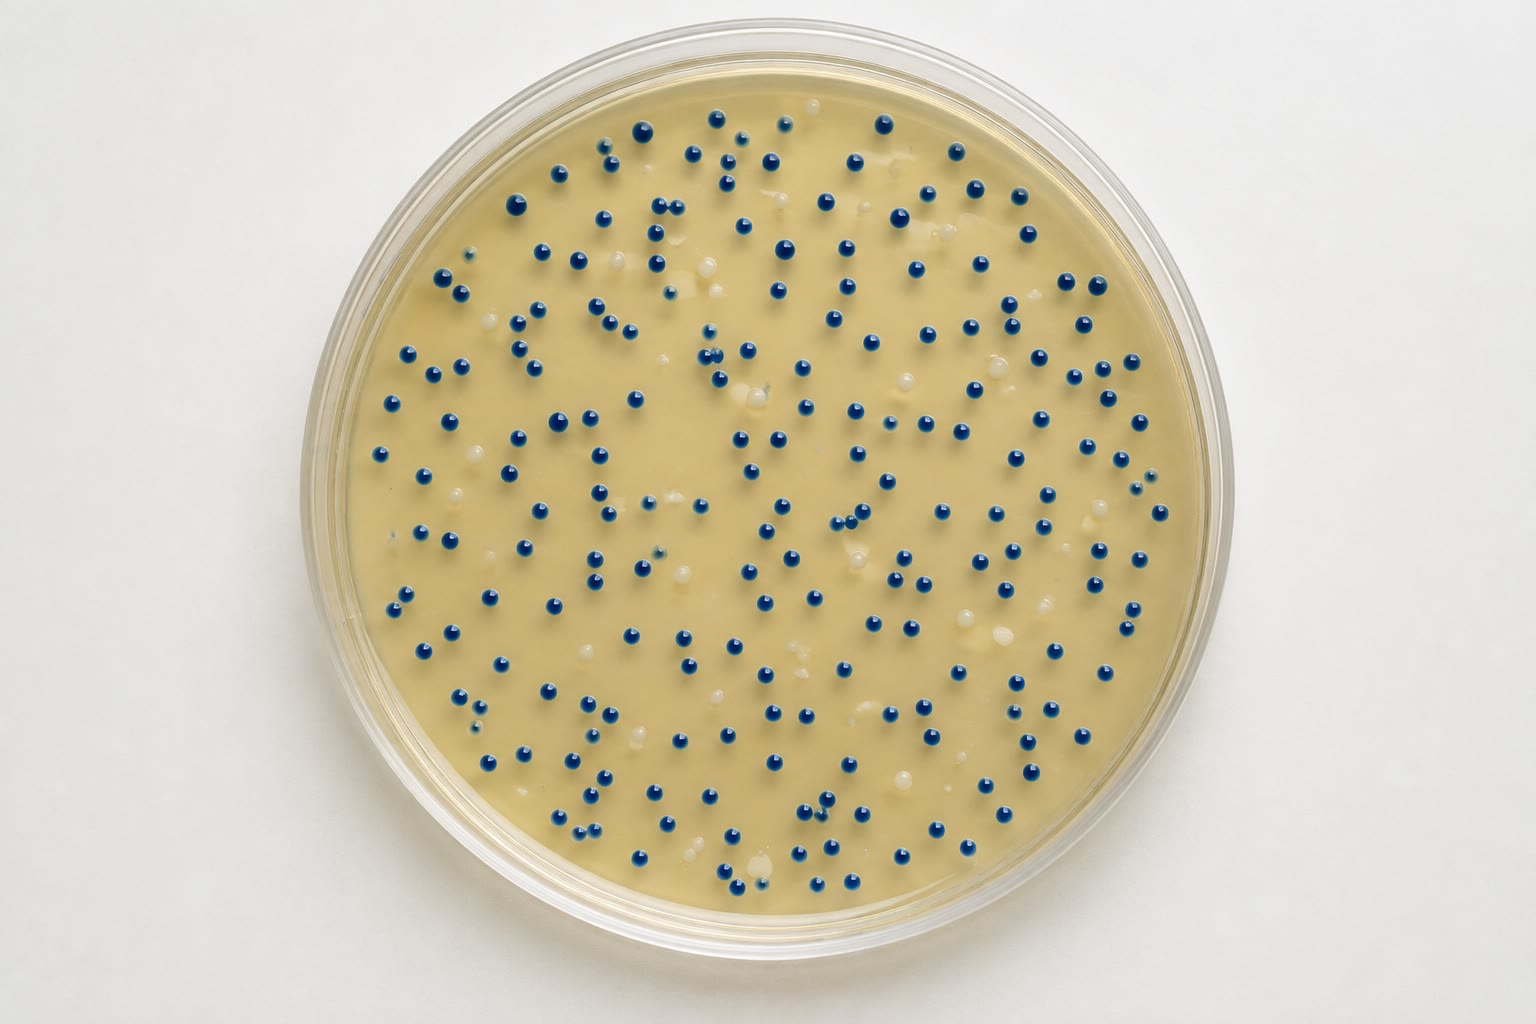
\includegraphics[width=0.46\linewidth]{images/book3/ai/b3-20-xgal-plate.jpg}

{\small 让 lac \omterm{def:b1:expression-control:operon}{操纵子}可见：含 X-gal 的平板上的菌落，
X-gal 是一种无色\omterm{def:b1:enzymes:enzyme}{底物}，$\beta$-半乳糖苷酶可使其显蓝色。
蓝色菌落表达 \emph{lacZ}；白色菌落携带受损\omterm{def:b1:genomes:gene}{基因}——
这一报告\omterm{def:b1:genomes:gene}{基因}曾被用于上千次实验。}
\end{omfigure}

\begin{method}[预测 lac 表型]\label{met:b1:expression-control:lacphenotype}
\begin{enumerate}
  \item 写出该区域每个拷贝的\omterm{def:b1:genomes:gene}{基因}型：$I$、$P$、$O$、
        $Z$（$^+$ 正常，$^-$ 失活，$O^c$ 组成型\omterm{def:b1:expression-control:operon}{操纵基因}，
        $I^s$ 超\omterm{def:b1:expression-control:operon}{阻遏蛋白}）。
  \item \omterm{def:b1:expression-control:operon}{阻遏蛋白}以反式作用：任一位置的一个 $I^+$ 即可阻遏
        每个正常的\omterm{def:b1:expression-control:operon}{操纵基因}；$I^s$ 无论诱导物如何都会阻遏。
  \item \omterm{def:b1:expression-control:operon}{操纵基因}与\omterm{def:b1:gene-expression:transcription}{启动子}以顺式作用：$O^c$ 仅释放
        其自身 \omterm{def:b1:nucleic-acids:chain}{DNA} 上的 $Z$；$P^-$ 只使自身\omterm{def:b1:genomes:gene}{基因}沉默。
  \item 在有、无诱导物时，分别检测每个 $Z^+$ \omterm{def:b1:genomes:gene}{基因}是否被转录；
        据此表型为可诱导、组成型或
        不可诱导。随后加入葡萄糖：无环 AMP--CAP 时，
        无论\omterm{def:b1:expression-control:operon}{阻遏蛋白}如何，转录水平都很低。
\end{enumerate}
\end{method}

\begin{example}[两个部分二倍体]\label{ex:b1:expression-control:diploids}
$I^-\,O^+\,Z^+ / I^+\,O^+\,Z^-$：$I^+$ 拷贝产生\omterm{def:b1:expression-control:operon}{阻遏蛋白}，
它结合 $O^+$（紧邻 $Z^+$）；可诱导——突变已被互补。
$I^+\,O^c\,Z^+ / I^+\,O^+\,Z^-$：唯一有功能的 $Z$
位于\omterm{def:b1:expression-control:operon}{阻遏蛋白}无法结合的\omterm{def:b1:expression-control:operon}{操纵基因}之后；组成型——
另一拷贝上正常的\omterm{def:b1:expression-control:operon}{操纵基因}无法提供帮助，因为它只控制
损坏的 $Z$。
\end{example}

\section{细菌的其他策略}

\begin{proposition}[阻遏、衰减与 sigma 因子]\label{prop:b1:expression-control:trp}
\index{trp 操纵子}\index{衰减}\index{sigma 因子}
生物合成\omterm{def:b1:expression-control:operon}{操纵子}的调控方向恰好相反：
\emph{trp \omterm{def:b1:expression-control:operon}{操纵子}}含有五个用于合成色氨酸的\omterm{def:b1:genomes:gene}{基因}，
除非色氨酸存在，否则会被转录——色氨酸与 trp
\omterm{def:b1:expression-control:operon}{阻遏蛋白}结合，并\emph{使其能够}结合\omterm{def:b1:expression-control:operon}{操纵基因}（一种共阻遏物）。
第二种更精细的调控，\emph{衰减}，利用了
细菌中转录与翻译的偶联：mRNA 起始段编码一个短肽，
该肽含有两个相连的色氨酸；若
负载色氨酸的 tRNA 充足，\omterm{def:b1:gene-expression:ribosome}{核糖体}便迅速翻译它，
其后的 \omterm{def:b1:nucleic-acids:chain}{RNA} 折叠成终止子发夹，使
聚合酶在这些\omterm{def:b1:genomes:gene}{基因}之前停止；若色氨酸匮乏，\omterm{def:b1:gene-expression:ribosome}{核糖体}
在色氨酸\omterm{def:b1:gene-expression:code}{密码子}处停滞，\omterm{def:b1:nucleic-acids:chain}{RNA} 以另一方式折叠，
使转录继续进行。细菌还能成组地切换\omterm{def:b1:genomes:gene}{基因}，
通过更换其聚合酶的 $\sigma$ 亚基：
热激 $\sigma$ 因子将其引向伴侣蛋白\omterm{def:b1:genomes:gene}{基因}的\omterm{def:b1:gene-expression:transcription}{启动子}；
孢子形成 $\sigma$ 因子则引向孢子形成相关\omterm{def:b1:genomes:gene}{基因}的\omterm{def:b1:gene-expression:transcription}{启动子}。
\end{proposition}

\section{真核生物中的调控}

\begin{definition}[转录因子、增强子]\label{def:b1:expression-control:enhancer}
\index{转录因子}\index{增强子}
在真核生物中，\omterm{def:b1:nucleic-acids:chain}{RNA} 聚合酶从不自行启动：\omterm{def:b1:gene-expression:transcription}{启动子}处的
基本转录因子（见\cref{ch:b1:gene-expression}）招募它，
速率由\emph{转录因子}决定，它们结合于
\emph{调控序列}——一些靠近\omterm{def:b1:gene-expression:transcription}{启动子}，许多在
\emph{增强子}中，它们可位于数千个\omterm{thm:b1:nucleic-acids:helix}{碱基对}之外，
位于上游、下游或\omterm{def:b1:genomes:gene}{内含子}中，方向任意，并以
\emph{成环}方式作用，使结合其上的因子经由中介蛋白
与\omterm{def:b1:gene-expression:transcription}{启动子}的复合体相接触。转录因子
是\omterm{prop:b1:flowering-plant-organization:modular}{模块化}的：一个\emph{\omterm{def:b1:nucleic-acids:chain}{DNA} 结合结构域}，用于\omterm{prop:b1:water-small-molecules:weak}{识别}短
序列（螺旋-转角-螺旋、锌指、亮氨酸拉链家族），
和\emph{激活结构域}或\emph{抑制结构域}，用以招募或
阻断转录机器。只有当正确的因子\emph{组合}存在时，\omterm{def:b1:genomes:gene}{基因}才被读取：
数百种因子以组合形式
控制两万个\omterm{def:b1:genomes:gene}{基因}。
\end{definition}

\begin{omfigure}
\begin{tikzpicture}[font=\footnotesize, >=Stealth, line cap=round]
  % DNA with enhancer far upstream, looped to promoter
  \draw[very thick, gray] (0,0) -- (2.2,0) .. controls (3.2,0) and (3.4,2.6) .. (5.0,2.6) .. controls (6.6,2.6) and (6.8,0) .. (7.8,0) -- (12.5,0);
  \fill[omExo!60] (0.4,-0.2) rectangle (2.0,0.2); \node[anchor=north, font=\scriptsize] at (1.2,-0.25) {增强子（距离 \qtyrange{1}{100}{kb}）};
  \fill[omProp!50] (8.0,-0.2) rectangle (9.4,0.2); \node[anchor=north, font=\scriptsize] at (8.7,-0.25) {启动子};
  \fill[omDef!60] (9.5,-0.2) rectangle (12.3,0.2); \node[anchor=north, font=\scriptsize] at (10.9,-0.25) {基因};
  % looped enhancer brought near promoter: draw factors at the loop apex near promoter? Simplify: activators on enhancer, mediator bridging
  \node[draw, thick, fill=omExo!30, rounded corners=3pt, inner sep=2pt] (act) at (1.2,0.75) {激活剂};
  \node[draw, thick, fill=omThm!25, rounded corners=3pt, inner sep=2pt, align=center] (med) at (5.0,1.5) {中介复合体};
  \node[draw, thick, fill=omProp!30, rounded corners=3pt, inner sep=2pt, align=center] (pol) at (8.7,0.85) {通用因子 \\ + 聚合酶};
  \draw[thick, omExo!80!black] (act) -- (2.4,1.2) -- (med);
  \draw[thick, omThm] (med) -- (pol);
  \node[anchor=north, align=center, gray] at (6.2,-1.0) {DNA 成环，使远处结合的因子接触启动子复合体；\\ 只有当正确的因子组合结合时，基因才被读取};
\end{tikzpicture}

{\small \omterm{def:b1:expression-control:enhancer}{增强子}的作用。结合于远处\omterm{def:b1:expression-control:enhancer}{增强子}上的激活剂，
借 \omterm{def:b1:nucleic-acids:chain}{DNA} 成环被带到\omterm{def:b1:gene-expression:transcription}{启动子}附近，中介复合体
将其信号传递给聚合酶。}
\end{omfigure}

\begin{proposition}[染色质是调控的一部分]\label{prop:b1:expression-control:chromatin}
\index{组蛋白乙酰化}\index{DNA 甲基化}
被包裹于\omterm{def:b1:genomes:nucleosome}{核小体}中、压缩成异\omterm{def:b1:genomes:nucleosome}{染色质}的\omterm{def:b1:genomes:gene}{基因}无法被读取：
因子无法接近它。激活剂招募能使\omterm{def:b1:genomes:nucleosome}{组蛋白}
\emph{乙酰化}的酶，使其与 \omterm{def:b1:nucleic-acids:chain}{DNA} 的结合松弛，
并将该区域标记为开放；阻遏因子招募能去除乙酰基的酶，
并添加使\omterm{def:b1:genomes:nucleosome}{染色质}压缩的标记。添加到\omterm{def:b1:gene-expression:transcription}{启动子}胞\omterm{def:b1:nucleic-acids:nucleotide}{嘧啶}上的甲基
使其长期沉默，这些标记在复制时被复制，
因此\omterm{def:b1:cell-unit-of-life:cell}{细胞}开放与关闭\omterm{def:b1:genomes:gene}{基因}的模式可遗传给其子\omterm{def:b1:cell-unit-of-life:cell}{细胞}——
肝\omterm{def:b1:cell-unit-of-life:cell}{细胞}的子\omterm{def:b1:cell-unit-of-life:cell}{细胞}仍为肝\omterm{def:b1:cell-unit-of-life:cell}{细胞}，正是依靠这种记忆（这些
\emph{表观遗传}机制在本科三年级分册中
深入讨论）。
\end{proposition}
\begin{proof}[证据]
在果蝇幼虫的巨型多线\omterm{def:b1:genomes:genome}{染色体}中（每条\omterm{def:b1:genomes:genome}{染色体}有一千个并排拷贝，
并带有条带），正在转录的\omterm{def:b1:genomes:gene}{基因}以\emph{膨泡}的形式出现，
即\omterm{def:b1:genomes:nucleosome}{染色质}展开之处；促使蜕皮的激素——蜕皮激素，
使一组特定的膨泡在数分钟内出现，其他膨泡则在数小时后
按固定顺序出现——转录被直接观察到，
并由信号开启。通过\omterm{def:b1:genomes:genome}{染色体}重排移至异\omterm{def:b1:genomes:nucleosome}{染色质}旁的\omterm{def:b1:genomes:gene}{基因}，
在某些\omterm{def:b1:cell-unit-of-life:cell}{细胞}中被沉默，在另一些\omterm{def:b1:cell-unit-of-life:cell}{细胞}中则不被沉默，
且这一状态可遗传给其子\omterm{def:b1:cell-unit-of-life:cell}{细胞}。
\end{proof}

\begin{omfigure}
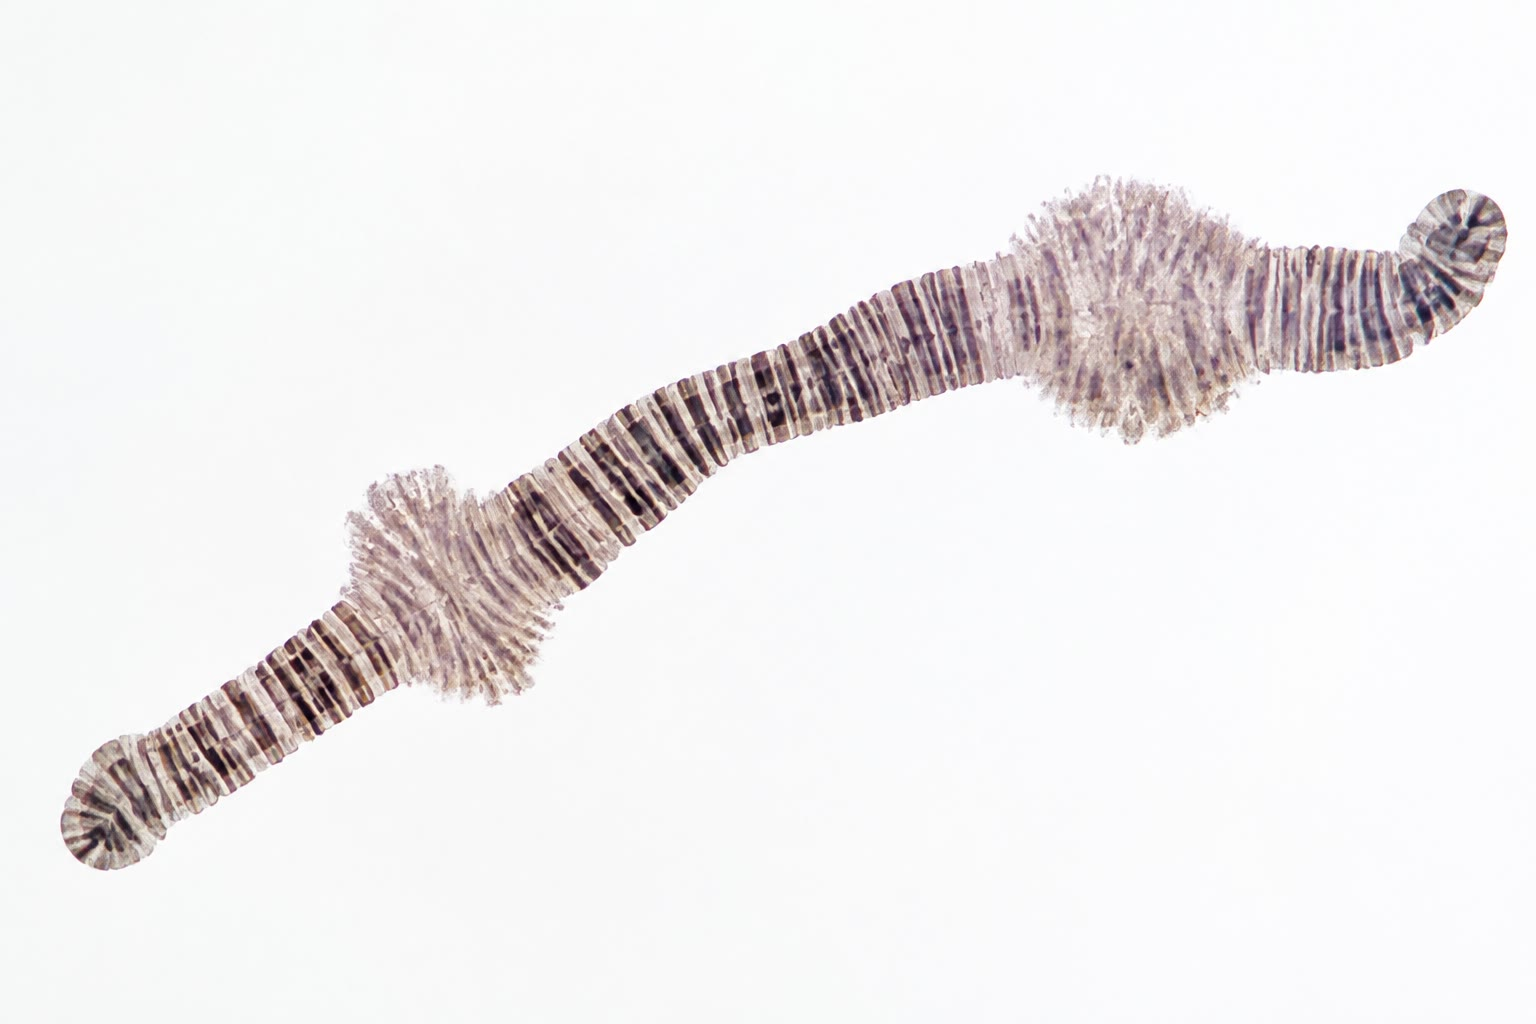
\includegraphics[width=0.56\linewidth]{images/book3/ai/b3-20-polytene-chromosome.jpg}

{\small 取自果蝇唾液腺的一条多线\omterm{def:b1:genomes:genome}{染色体}，
具有条带，其中两处膨泡为\omterm{def:b1:genomes:nucleosome}{染色质}已打开以进行转录之处。
膨泡随\omterm{def:b1:genomes:gene}{基因}的开启与关闭而出现与消失。}
\end{omfigure}

\begin{example}[信号变为表达模式]\label{ex:b1:expression-control:steroid}
皮质醇进入肝\omterm{def:b1:cell-unit-of-life:cell}{细胞}并结合其受体，该受体是一种在\omterm{def:b1:cell-unit-of-life:cell}{细胞质}中
保持失活的\omterm{def:b1:expression-control:enhancer}{转录因子}；复合体进入\omterm{def:b1:eukaryotic-cell:nucleus}{细胞核}，结合于约一百个\omterm{def:b1:genomes:gene}{基因}附近
存在的一段十五碱基序列上——其中包括\omterm{def:b1:biosyntheses-integration:gluconeogenesis}{糖异生}\omterm{def:b1:genomes:gene}{基因}
（见\cref{ch:b1:biosyntheses-integration}）——并招募乙酰化酶与中介复合体：
一小时内，葡萄糖合成的酶即开始合成。同一种激素作用于淋巴\omterm{def:b1:cell-unit-of-life:cell}{细胞}时，
其开放的\omterm{def:b1:genomes:nucleosome}{染色质}暴露出的是另一组这些序列，
从而开启了可杀死该\omterm{def:b1:cell-unit-of-life:cell}{细胞}的\omterm{def:b1:genomes:gene}{基因}。
一个信号，一种受体，两种反应：
区别在于哪些\omterm{def:b1:genomes:gene}{基因}可被接近。
\end{example}

\section{转录之后，以及身体的形成}

\begin{proposition}[启动子之外的调控]\label{prop:b1:expression-control:posttranscriptional}
\index{mRNA 稳定性}
\omterm{def:b1:cell-unit-of-life:prokeuk}{真核细胞}还决定转录本如何剪接（可变剪接使同一\omterm{def:b1:genomes:gene}{基因}在肌肉与脑中
产生不同的\omterm{def:b1:proteins:peptide}{蛋白质}）、是否输出、存活多久（半衰期从数分钟（调控蛋白的
信使 \omterm{def:b1:nucleic-acids:chain}{RNA}）到数天（血红蛋白的信使 \omterm{def:b1:nucleic-acids:chain}{RNA}）不等，由非翻译区中结合\omterm{def:b1:proteins:peptide}{蛋白质}
与小分子调控 \omterm{def:b1:nucleic-acids:chain}{RNA} 的序列决定），以及是否被翻译（缺铁的\omterm{def:b1:cell-unit-of-life:cell}{细胞}会通过
与铁蛋白信使 \omterm{def:b1:nucleic-acids:chain}{RNA} 的 $5'$ 端结合的\omterm{def:b1:proteins:peptide}{蛋白质}阻止其翻译，
而在有铁时该蛋白释放之）。
\omterm{def:b1:proteins:peptide}{蛋白质}一经合成，便由修饰与降解加以调控（见\cref{ch:b1:enzymes}）。
越往后的每一层级都比前一层级更快、
更局部，也更昂贵：
转录决定\omterm{def:b1:cell-unit-of-life:cell}{细胞}能够做什么，
后续各层级则决定
\omterm{def:b1:cell-unit-of-life:cell}{细胞}此刻正在做什么。
\end{proposition}

\begin{proposition}[差异表达造就身体]\label{prop:b1:expression-control:differentiation}
\index{分化}
多\omterm{def:b1:cell-unit-of-life:cell}{细胞}生物的每个\omterm{def:b1:cell-unit-of-life:cell}{细胞}都携带相同的\omterm{def:b1:genomes:genome}{基因组}，
\omterm{def:b1:cell-unit-of-life:cell}{细胞}之间的差异在于其表达\omterm{def:b1:genomes:genome}{基因组}的不同子集。
\emph{管家}\omterm{def:b1:genomes:gene}{基因}——数千个，负责代谢、\omterm{def:b1:gene-expression:ribosome}{核糖体}与\omterm{def:b1:eukaryotic-cell:cytoskeleton}{细胞骨架}——
在每个\omterm{def:b1:cell-unit-of-life:cell}{细胞}中都开启；
其余\omterm{def:b1:genomes:gene}{基因}则在某些\omterm{def:b1:cell-unit-of-life:cell}{细胞}中开启、在另一些\omterm{def:b1:cell-unit-of-life:cell}{细胞}中关闭，
这取决于各\omterm{def:b1:cell-unit-of-life:cell}{细胞}所携带的\omterm{def:b1:expression-control:enhancer}{转录因子}组合，以及其所继承的\omterm{def:b1:genomes:nucleosome}{染色质}状态。
红\omterm{def:b1:cell-unit-of-life:cell}{细胞}前体开启珠蛋白\omterm{def:b1:genomes:gene}{基因}，几乎关闭其他一切；
\omterm{def:b1:body-plans-tissues:nervous}{神经元}则开启其\omterm{def:b1:membranes-transport:transporters}{通道蛋白}，并且不再分裂。
\emph{分化}是获得稳定表达模式的过程，
而\emph{发育}（见本科二年级分册）是
\omterm{def:b1:cell-unit-of-life:cell}{细胞}间的信号将这些模式
设定于正确位置的过程。
\end{proposition}
\begin{proof}[证据]
从已分化的蛙\omterm{def:b1:cell-unit-of-life:cell}{细胞}中取出\omterm{def:b1:eukaryotic-cell:nucleus}{细胞核}，放入去除了自身
\omterm{def:b1:eukaryotic-cell:nucleus}{细胞核}的卵\omterm{def:b1:cell-unit-of-life:cell}{细胞}中，即可指导发育出一只完整的蝌蚪
（格登，1962 年；见高中分册回顾）：已分化的\omterm{def:b1:cell-unit-of-life:cell}{细胞}
并未丢失任何\omterm{def:b1:genomes:gene}{基因}，只是将其关闭，而卵\omterm{def:b1:cell-unit-of-life:cell}{细胞}的\omterm{def:b1:cell-unit-of-life:cell}{细胞质}
重新设定了这些开关。某一\omterm{def:b1:cell-unit-of-life:cell}{细胞}类型的\omterm{def:b1:proteins:peptide}{蛋白质}在凝胶上分离后，
与另一类型的不同；其信使 \omterm{def:b1:nucleic-acids:chain}{RNA} 经测序后，
是该\omterm{def:b1:cell-unit-of-life:cell}{细胞}特有的\omterm{def:b1:genomes:genome}{基因组}子集；并且，将少量\omterm{def:b1:expression-control:enhancer}{转录因子}
导入皮肤\omterm{def:b1:cell-unit-of-life:cell}{细胞}，
即可使其重编程为干\omterm{def:b1:cell-unit-of-life:cell}{细胞}或\omterm{def:b1:body-plans-tissues:nervous}{神经元}。
\end{proof}

\begin{example}[一个基因在两个器官中被读取]\label{ex:b1:expression-control:twoorgans}
催化由葡萄糖-6-磷酸生成葡萄糖的酶的\omterm{def:b1:genomes:gene}{基因}
仅在肝脏和肾脏中表达，在其他\omterm{def:b1:body-plans-tissues:tissue}{组织}中不表达：其
\omterm{def:b1:gene-expression:transcription}{启动子}带有仅存在于这两种\omterm{def:b1:mammal-organization:organ}{器官}中的因子的结合位点，在其他
\omterm{def:b1:cell-unit-of-life:cell}{细胞}中其\omterm{def:b1:gene-expression:transcription}{启动子}发生甲基化，\omterm{def:b1:genomes:nucleosome}{染色质}关闭。肌肉
\omterm{def:b1:cell-unit-of-life:cell}{细胞}虽携带完整的该\omterm{def:b1:genomes:gene}{基因}，却无法将葡萄糖释放入血液
（见\cref{ch:b1:biosyntheses-integration}）——并非因缺少该\omterm{def:b1:genomes:gene}{基因}，
而是因为该\omterm{def:b1:genomes:gene}{基因}未被读取。\omterm{def:b1:genomes:genome}{基因组}是相同的；
表达模式决定\omterm{def:b1:mammal-organization:organ}{器官}。
\end{example}

\section{练习}

\begin{exercise}[$\star$]\label{exo:b1:expression-control:1}
写出 lac \omterm{def:b1:expression-control:operon}{操纵子}的组成元件，并给出该\omterm{def:b1:expression-control:operon}{操纵子}
在有、无乳糖及有、无葡萄糖时的状态。
\end{exercise}

\begin{exercise}[$\star$]\label{exo:b1:expression-control:2}
解释反式作用的\omterm{def:b1:genomes:gene}{基因}产物与顺式作用的位点之间的区别，
并各以\omterm{def:b1:expression-control:operon}{操纵子}中的一个例子加以说明。
\end{exercise}

\begin{exercise}[$\star$]\label{exo:b1:expression-control:3}
由\omterm{def:b1:expression-control:cap}{二次生长}图读出延迟期的时长，以及
在每种糖上的倍增时间。
\end{exercise}

\begin{exercise}[$\star$]\label{exo:b1:expression-control:4}
给出\omterm{def:b1:expression-control:enhancer}{增强子}、\omterm{def:b1:expression-control:enhancer}{转录因子}和管家\omterm{def:b1:genomes:gene}{基因}的定义。
\end{exercise}

\begin{exercise}[$\star\star$]\label{exo:b1:expression-control:5}
给出下列各菌株的表型（可诱导的、组成型的、不可诱导的）：$I^-$；
$O^c$；$I^s$；$I^-\,O^+\,Z^+ / I^+\,O^+\,Z^+$；$I^s\,O^+\,Z^+ /
I^+\,O^+\,Z^+$；$I^+\,O^c\,Z^- / I^+\,O^+\,Z^+$。
\end{exercise}

\begin{exercise}[$\star\star$]\label{exo:b1:expression-control:6}
比较 lac \omterm{def:b1:expression-control:operon}{操纵子}与 trp \omterm{def:b1:expression-control:operon}{操纵子}：小分子对
各自\omterm{def:b1:expression-control:operon}{阻遏蛋白}的作用，以及两者的调控逻辑为何相反。
\end{exercise}

\begin{exercise}[$\star\star$]\label{exo:b1:expression-control:7}
某突变体不能合成环 AMP。预测其在葡萄糖上、仅在乳糖上
及两者同时存在时的生长情况，并给出各情况下 $\beta$-半乳糖苷酶的
水平。
\end{exercise}

\begin{exercise}[$\star\star$]\label{exo:b1:expression-control:8}
试从\omterm{def:b1:cell-unit-of-life:prokeuk}{真核细胞}的结构出发，解释为何真核生物中
不可能发生衰减。
\end{exercise}

\begin{exercise}[$\star\star$]\label{exo:b1:expression-control:9}
将一\omterm{def:b1:expression-control:enhancer}{增强子}从其\omterm{def:b1:genomes:gene}{基因}上游 \qty{5}{kb} 处
移至其\omterm{def:b1:genomes:gene}{基因}下游 \qty{5}{kb} 处并使其倒置；该\omterm{def:b1:genomes:gene}{基因}仍被表达。
解释这说明\omterm{def:b1:expression-control:enhancer}{增强子}如何发挥作用。
\end{exercise}

\begin{exercise}[$\star\star\star$]\label{exo:b1:expression-control:10}
五千个 $\beta$-半乳糖苷酶四聚体，每个由 \qty{4096}{}
个残基组成，需要多少个 \omterm{def:b1:water-small-molecules:atp}{ATP}（每个残基四个）？
\omterm{def:b1:cell-unit-of-life:cell}{细胞}每代的预算约为 \qty{1e10}{} \omterm{def:b1:water-small-molecules:atp}{ATP}。计算
组成型突变体的生长劣势，以及其在混合种群中
所占份额从二分之一降至
百分之一所需的世代数。
\end{exercise}

\begin{exercise}[$\star\star\star$]\label{exo:b1:expression-control:11}
比较同一人的肝\omterm{def:b1:cell-unit-of-life:cell}{细胞}与\omterm{def:b1:body-plans-tissues:nervous}{神经元}：二者\omterm{def:b1:genomes:genome}{基因组}相同、
\omterm{def:b1:proteins:peptide}{蛋白质}不同，且肝\omterm{def:b1:cell-unit-of-life:cell}{细胞}每次分裂
产生的仍是肝\omterm{def:b1:cell-unit-of-life:cell}{细胞}。请结合\omterm{def:b1:genomes:nucleosome}{染色质}、因子以及表观标记的遗传，
说明这种差异是如何形成的，又是如何维持的。
\end{exercise}

\begin{exercise}[$\star\star\star$]\label{exo:b1:expression-control:12}
“细菌读取其所处的\omterm{def:b1:organism-environment:organism}{环境}，体内的\omterm{def:b1:cell-unit-of-life:cell}{细胞}则读取其
历史。”请以一段文字讨论两类调控，比较它们的
信号、时间尺度与可逆性。
\end{exercise}

\section{问题：二次生长}

\begin{problem}[{周末问题——莫诺的两相生长曲线
逐细胞重建：葡萄糖耗尽，乳糖诱导，
统计酶的数量，预测突变体，并计算调控的代价，
最后归结于 $\beta$-半乳糖苷酶的诱导倍数}]
\label{pb:b1:expression-control:1}
一份 \emph{E. coli} 培养物起始于每毫升 $10^7$ 个\omterm{def:b1:cell-unit-of-life:cell}{细胞}的密度，
培养基中含 \qty{0.5}{mmol/L} 葡萄糖和 \qty{1.0}{mmol/L} 乳糖。
在葡萄糖上\omterm{def:b1:cell-unit-of-life:cell}{细胞}每 \qty{20}{min} 倍增一次，在乳糖上
每 \qty{30}{min} 倍增一次；每次分裂，一个\omterm{def:b1:cell-unit-of-life:cell}{细胞}需要 \qty{1.5e-12}{g} 的糖，
（葡萄糖的摩尔质量为 \qty{180}{g/mol}；乳糖为 \qty{342}{g/mol}，
按两个葡萄糖计）。未诱导的\omterm{def:b1:cell-unit-of-life:cell}{细胞}含有 5 个
$\beta$-半乳糖苷酶分子；充分诱导后为 \num{5000} 个。诱导需要
\qty{30}{min}。该酶为四聚体，共含 $4\times 1024$ 个残基；
每个残基耗 4 个 \omterm{def:b1:water-small-molecules:atp}{ATP}；\omterm{def:b1:cell-unit-of-life:cell}{细胞}每次分裂的 \omterm{def:b1:water-small-molecules:atp}{ATP} 预算为 $10^{10}$，
其\omterm{def:b1:proteins:peptide}{蛋白质}量为 $\qty{1.5e-13}{g}$（每残基 \qty{110}{Da}）。

\medskip
\noindent\textbf{第一部分——葡萄糖阶段。}
\begin{enumerate}
  \item 计算每毫升可用葡萄糖的质量（以克计）。
  \item 每毫升的葡萄糖能支持多少次分裂？
  \item 从 $10^7$ 个\omterm{def:b1:cell-unit-of-life:cell}{细胞}出发，葡萄糖耗尽时，
        共有多少个\omterm{def:b1:cell-unit-of-life:cell}{细胞}？（每次分裂产生一个新\omterm{def:b1:cell-unit-of-life:cell}{细胞}。）
  \item 这相当于多少次倍增，葡萄糖阶段的
        持续时间有多长？
  \item 在此阶段，lac \omterm{def:b1:expression-control:operon}{操纵子}处于什么状态，
        从分子水平（\omterm{def:b1:expression-control:operon}{阻遏蛋白}与 CAP）看，原因何在？
\end{enumerate}

\medskip
\noindent\textbf{第二部分——开关。}
\begin{enumerate}[resume]
  \item 葡萄糖耗尽后，\omterm{def:b1:cell-unit-of-life:cell}{细胞}内有什么物质上升，
        它与什么结合？
  \item 乳糖一直存在。为什么在葡萄糖阶段，\omterm{def:b1:expression-control:operon}{操纵子}仍然
        几乎关闭？
  \item 在 \qty{30}{min} 的延滞期内，每个\omterm{def:b1:cell-unit-of-life:cell}{细胞}合成 \num{5000}
        个酶分子。计算每个\omterm{def:b1:cell-unit-of-life:cell}{细胞}每秒合成的酶分子数，
        以及每秒合成的残基数。
  \item 一个\omterm{def:b1:cell-unit-of-life:cell}{细胞}含有 \num{20000} 个\omterm{def:b1:gene-expression:ribosome}{核糖体}，每个\omterm{def:b1:gene-expression:ribosome}{核糖体}每秒合成 \qty{20}{}
        个残基。在延滞期内，有多大比例的翻译用于合成
        $\beta$-半乳糖苷酶？
  \item 计算 \num{5000} 个四聚体的质量，以及它们
        占\omterm{def:b1:cell-unit-of-life:cell}{细胞}\omterm{def:b1:proteins:peptide}{蛋白质}的比例。
  \item 计算诱导倍数。
  \item 为什么通透酶（\emph{lacY}）与酶本身同样是
        利用乳糖生长所必需的？若给予乳糖，\emph{lacY}$^-$
        突变体会出现什么情况？
\end{enumerate}

\medskip
\noindent\textbf{第三部分——乳糖阶段。}
\begin{enumerate}[resume]
  \item 以葡萄糖当量计，计算每毫升可用的乳糖
        的质量（以克计）。
  \item 它还能支持多少次分裂，最终
        \omterm{def:b1:cell-unit-of-life:cell}{细胞}数是多少？
  \item 乳糖阶段持续多长时间？
  \item 画出时间线：葡萄糖阶段、延滞期、乳糖阶段、总时间。
  \item 解释为什么在乳糖上的倍增时间更长
        （两个原因：一个与酶的步骤有关，一个与通透酶有关）。
\end{enumerate}

\medskip
\noindent\textbf{第四部分——突变体与代价。}
\begin{enumerate}[resume]
  \item 一个 $I^-$ 突变体：描述它在相同培养基上的生长曲线，
        以及其酶水平在整个过程中的变化。
  \item 一个 CAP$^-$ 突变体：描述其曲线和酶水平。
  \item 一个 $O^c$ 突变体在仅含乳糖的培养基中：与野生型有何差异？
        仅含葡萄糖时呢？
  \item 计算合成 \num{5000} 个四聚体每代所需的 \omterm{def:b1:water-small-molecules:atp}{ATP} 代价，
        以及其占\omterm{def:b1:cell-unit-of-life:cell}{细胞}预算的比例。
  \item 若该比例使世代时间以相同比例延长，
        则 $I^-$ 突变体在葡萄糖上的生长速率
        比野生型落后多少？
  \item 起始个体数相等，在葡萄糖上经过多少代后，
        突变体占群体的十分之一？（$r^n =
        0.1/0.9$，其中 $r$ 为每代生长速率之比，
        即 $2^{-\delta}$，其中 $\delta$ 为以倍增数计的延滞。）
  \item 解释为什么尽管如此，$I^-$ 突变体在
        以乳糖培养的实验室菌株中仍然很常见。
  \item 陈述结果：
        $\beta$-半乳糖苷酶的诱导倍数、无必要地合成它所付出的
        以占 \omterm{def:b1:water-small-molecules:atp}{ATP} 预算的比例表示的代价，以及双相实验的
        总时间。
\end{enumerate}
\end{problem}
